\section{Risultati ottenuti}
\subsection{Metriche utilizzate per detection su singole immagini}
Nell'ambito della computer vision vengono tipicamente utilizzate due tipi di metriche per misurare due diverse proprietà:
\begin{itemize}
\item Corretta determinazione della posizione degli oggetti;
\item Rilevamento dell'esistenza degli oggetti nell'immagine e la loro corretta classificazione.
\end{itemize}
Le metriche utilizzate per misurare la bontà dei risultati del progetto sono F1, AP (Average Precision) e mAp (mean Average Precision) le quali misurano la seconda proprietà sopra elencata.
Prima di iniziare a descrivere le metriche è necessario definire alcuni concetti che saranno poi coinvolti per il calcolo dei valori delle metriche.
\subsubsection{Precision}
La precision misura l'accuratezza delle classificazioni ed indica la percentuale di classificazioni corrette sulla base di quelle totali e viene calcolata come:
\[
    precision = \frac{TP}{TP + FP}
\]
Dove TP (True Positives) è il numero di classificazioni corrette e FP (False Positives) è il numero di classificazioni errate. E' da sottolineare che se uno stesso elemento viene individuato più di una volta, solo la prima volta conterà come TP mentre il resto delle volte conterà come FP. Questa metrica fornisce un'idea sulla correttezza dei risultati.
\subsubsection{Recall}
La recall misura quanti oggetti sono stati individuati e classificati correttamente sulla base degli oggetti totali, viene calcolata come:
\[
    recall = \frac{TP}{TP + FN}
\]
Dove TP (True Positives) è sempre il numero di classificazioni corrette mentre FN (False Negatives) è il numero di di oggetti che non sono stati individuati ma che se sarebbe stato corretto individuare. Questa metrica fornisce un'idea sulla completezza dei risultati.
\subsubsection{F1}
F1 è una metrica che combina la precision con il recall e può essere interpretata come la media armonica tra la precision e la recall. Il valore massimo ottenibile è 1 raggiungibile nel caso in cui sia la precision che la recall siano pari ad 1 mentre il valore minimo è 0 ottenuto quando entrambe le metriche che lo compongono assumono valore pari a 0. Viene calcolato come:
\[
    F1 = 2 \times \frac{precision \times recall}{precision + recall}
\]
\subsubsection{Intersection over union}
L'intersection over union (IoU) misura il grado di sovrapposizione tra due aree e viene usato per misurare il grado di sovrapposizione tra la box dell'oggetto individuato e la box dell'oggetto reale. Viene calcolata come:
\[
    IoU = \frac{AI}{AU}
\]
Dove AI (Area dell'Intersezione) corrisponde all'area dell'intersezione tra le due bounding boxes e AU (Area dell'Unione) corrisponde all'area dell'unione tra le due bounding boxes.
Una label per essere considerata come corretta deve avere un valore di IoU maggiore di una soglia stabilità (per esempio 0.5).
\begin{figure}[H]
	\centering
	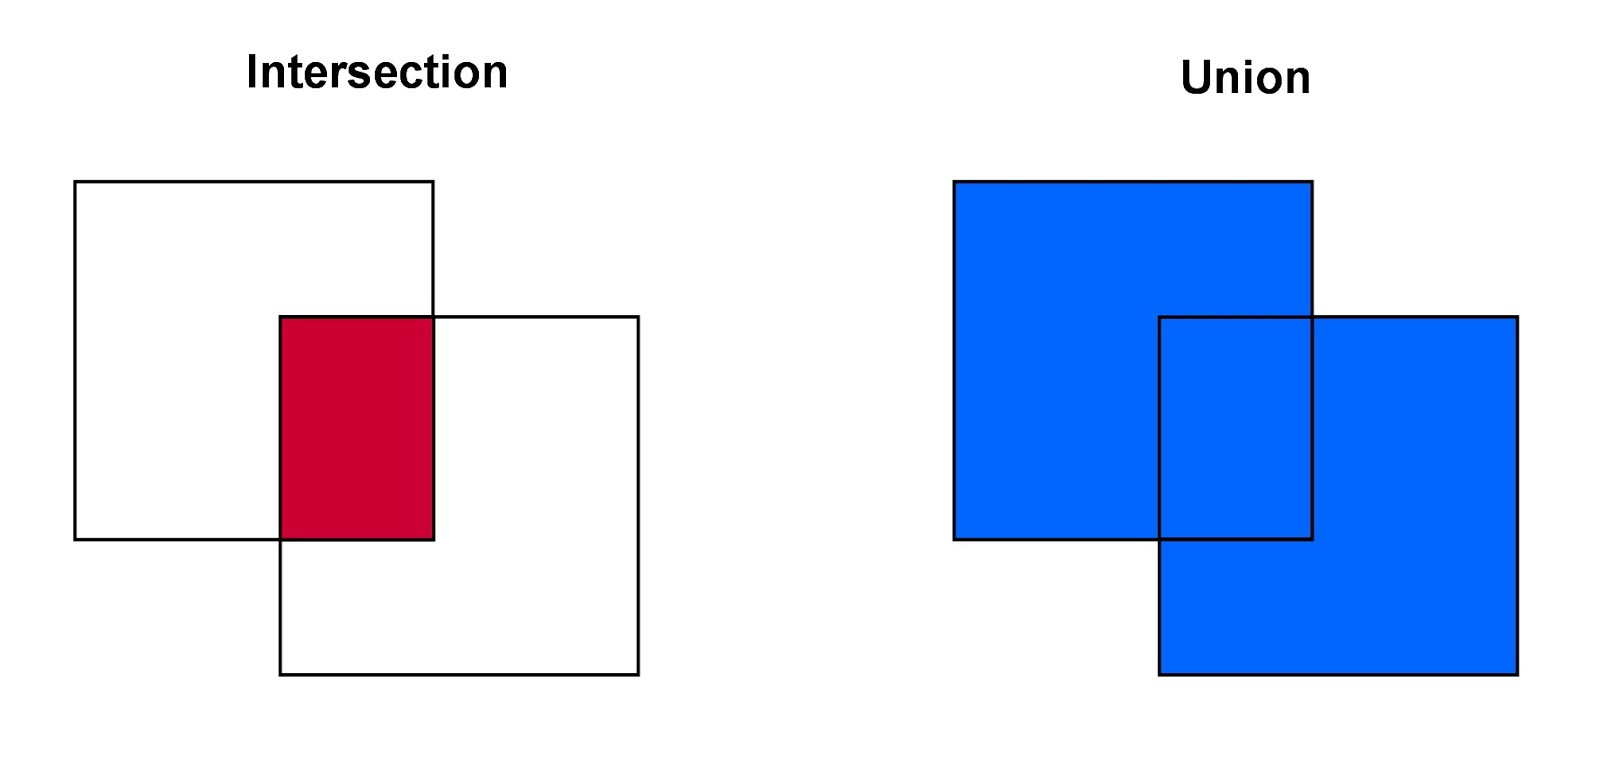
\includegraphics[width=0.5\linewidth]{images/unione-intersezione.jpg}
	\caption{Esempio di intersezione e di unione}
	\label{Esempio di intersezione e di unione}
\end{figure}
\subsubsection{Average Precision}
Un'altra delle metriche utilizzate è l'average precision (AP) e per calcolarla si fa la media delle precisioni di undici diversi valori di recall equamente distribuiti. Questa metrica viene applicata ad una sola categoria di elementi e viene calcolata tramite la seguente formula:
\[
    AP = \frac{1}{11}\sum_{Recall\ped{i}}^{} Precision(Recall\ped{i})
\]
Dove \textit{i}=[0, 0.1, 0.2, …, 1.0] in quanto 0 \textless =recall\textless =1. Inoltre la precisione di uno specifico valore di recall viene calcolata nel seguente modo:
\[
    Precision(Recall\ped{i}) = max\,Precision(Recall\ped{j}) \quad \textrm{and} \quad j>=i
\]
L'AP è un valore che riassume la forma della curva precision/recall per una data categoria.
\subsubsection{Mean Average Precision}
La mean average precision (mAP) è la media delle AP di tutte le categorie calcolata su diverse soglie di IoU:
\[
    mAP\ped{IoU=x\%} = \frac{1}{n}\sum_{i=0}^{n}AP\ped{i}
\]
Dove \textit{i} è il numero totale di categorie sulle quali è stata calcolata la propria AP e \textit{x} rappresenta diverse soglie di IoU.

\subsection{Dataset utilizzato per detection su singole immagini}
I test sono stati eseguiti su un dataset di immagini satellitari in alta risoluzione con circa 3000 pixels di altezza e 4000 di larghezza. Il modello di rete è stato allenato per riconoscere oggetti appartenenti alle sessanta categorie mostrate nella seguente tabella:

\subsubsection{Impostazione parametri detection}
Ogni immagine è stata suddivisa in regioni da 300x300 pixels.

\subsection{Risultati ottenuti nella detection su singole immagini}
\begin{center}
\begin{longtable}{|c|l|}
\caption{Lista delle categorie del dataset utilizzato per effettuare i test}
\label{lista categorie} \\

\hline \multicolumn{1}{|c|}{\textbf{Numero}} &\multicolumn{1}{c|}{\textbf{Categoria}} \\ \hline\endfirsthead

\hline \multicolumn{1}{|c|}{\textbf{Numero}} & \multicolumn{1}{c|}{\textbf{Categoria}} \\ \hline \endhead

\hline \multicolumn{2}{|c|}{{------ Continua nella pagina successiva ------}} \\ \hline
\endfoot

\hline \hline
\endlastfoot

1 & Fixed-wing Aircraft \\
2 & Small Aircraft \\
3 & Cargo Plane \\
4 & Helicopter \\
5 & Passenger Vehicle \\
6 & Small Car \\
7 & Bus \\
8 & Pickup Truck \\
9 & Utility Truck \\
10 & Truck \\
11 & Cargo Truck \\
12 & Truck w/Box \\
13 & Truck Tractor \\
14 & Trailer \\
15 & Truck w/Flatbed \\
16 & Truck w/Liquid \\
17 & Crane Truck \\
18 & Railway Vehicle \\
19 & Passenger Car \\
20 & Cargo Car \\
21 & Flat Car \\
22 & Tank car \\
23 & Locomotive \\
24 & Maritime Vessel \\
25 & Motorboat \\
26 & Sailboat \\
27 & Tugboat \\
28 & Barge \\
29 & Fishing Vessel \\
30 & Ferry \\
31 & Yacht \\
32 & Container Ship \\
33 & Oil Tanker \\
34 & Engineering Vehicle \\
35 & Tower Crane \\
36 & Container Crane \\
37 & Reach Stacker \\
38 & Straddle Carrier \\
39 & Mobile Crane \\
40 & Dump Truck \\
41 & Haul Truck \\
42 & Scraper/Tractor \\
43 & Front Loader/Bulldozer \\
44 & Excavator \\
45 & Cement Mixer \\
46 & Ground Grader \\
47 & Hut/Tent \\
48 & Shed \\
49 & Building \\
50 & Aircraft Hangar \\
51 & Damaged Building \\
52 & Facility \\
53 & Construction Site \\
54 & Vehicle Lot \\
55 & Helipad \\
56 & Storage Tank \\
57 & Shipping Container Lot \\
58 & Shipping Container \\
59 & Pylon \\
60 & Tower \\
\end{longtable}
\end{center}

\subsection{Metriche utilizzate per tracking su video}
L'obiettivo del tracking è quello di identificare tutti gli oggetti in un video e tracciarli nel tempo. Quest'ultimo compito viene svolto assegnando un ID unico a ciascun oggetto assicurandosi che esso rimanga lo stesso per tutta la durata del video. Di conseguenza nel tracking sono due gli aspetti fondamentali di cui tenere conto:
\begin{itemize}
\item Precisione con cui viene determinata la locazione di un oggetto;
\item Correttezza del tracciamento (anche in presenza di occultamento, perdita di qualità, etc...)
\end{itemize}
In seguito vengono descritte le metriche utilizzare per valutare la qualità del tracciamento.

\subsubsection{Mostly Tracked Trajectories}
Mostly Tracked Trajectories (MT), misura la percentuale di elementi, rispetto a quelli totali, che sono stati tracciati correttamente per almeno l'80\% della loro traiettoria. Indica quindi la correttezza del tracciamento, valori più alti sono considerati migliori.
\subsubsection{Mostly Lost Trajectories}
Mostly Lost Trajectories (ML), misura la percentuale di elementi, rispetto a quelli totali, che sono stati tracciati correttamente per non più del 20\% della loro traiettoria. Al contrario di MT, valori più bassi sono considerati migliori.
\subsubsection{ID switches}
ID switches (IDs), viene definito come il numero di volte che un oggetto tracciato cambia il suo ID assegnato. Questo può accadere per esempio nel momento in cui due elementi simili incrociano le loro traiettorie ed i trackers non sono in grado di distinguerli. Anche in questo caso, valori minori esprimono risultati migliori.
\subsubsection{Fragments}
Fragments (FM) conta il numero di volte che una traiettoria viene interrotta durante il tracciamento. Può accadere per esempio a seguito di un occultamento di un elemento, in questo caso un oggetto verrebbe momentaneamente perso e di conseguenza la sua traiettoria risulterebbe frammentata. Valori minori sono considerati migliori. 
\subsubsection{MOTP}
MOTP (Multiple Object Tracking Precision) rappresenta la capacità del sistema di tracking nello stimare con precisione la posizione degli elementi del video attraverso tutti i suoi frames. Viene calcolata nel seguente modo:
\[
MOTP = \frac{\sum_{t}^{}\sum_{i}^{}d\ped{t}\ap{i}}{\sum_{t}^{}c\ped{t}}
\]
Dove \textit{t}=[1,...,n] è l'indice dei frames del video ed \textit{n} è il numero di frames totali, \textit{i}=[1,...,\textit{c\ped{t}}] è l'indice delle associazioni detection-tracker effettuate nel frame \textit{t}, \textit{d\ped{t}\ap{i}} è la distanza tra la posizione reale dell'oggetto \textit{i} e la sua corrispondente posizione stimata nel frame \textit{t}, \textit{c\ped{t}} è il numero di associazioni detection-tracker effettuate nel frame \textit{t}.
\subsubsection{MOTA}
MOTA (Multiple Object Tracking Accuracy) fornisce una misura delle prestazioni del sistema di tracking nel riconoscere gli oggetti presenti nel video e costruire le loro traiettorie. Viene calcolata nel seguente modo:
\[
MOTA = 1-\frac{\sum_{t}^{}(fn\ped{t}+fp\ped{t}+mme\ped{t})}{\sum_{t}^{}g\ped{t}}
\]
Dove \textit{fn\ped{t}} è il numero di falsi negativi, fp\ped{t} è il numero di falsi positivi, mme\ped{t} è il numero di mismatches. Un mismatch avviene quando durante l'associazione detection-tracker un tracker viene associato ad una detection che rappresenta un oggetto diverso da quello associato nel frame precedente. Infine  \textit{g\ped{t}} è il numero di oggetti presenti nel frame \textit{t}.
\subsubsection{IDF1}
IDF1 è una metrica molto simile ad F1 utilizzata come metrica per singole immagini. Questa metrica applicata nell'ambito del tracking fornisce un bilanciamento tra la \textit{precision} media e la \textit{recall} media attraverso la loro media armonica. 
\[
IDF1 = \frac{2IDTP}{2IDTP+IDFP+IDFN}
\]
Dove IDTP, IDFP, IDFN rispettivamente sono la media del numero di detections avvenute correttamente, falsi positivi e falsi negativi calcolati su tutti i frames. 

\subsection{Dataset utilizzato per tracking su video}

\subsubsection{Impostazione parametri tracking}


\subsection{Risultati ottenuti nel tracking su video}